%!TeX root=../tese.tex
%("dica" para o editor de texto: este arquivo é parte de um documento maior)
% para saber mais: https://tex.stackexchange.com/q/78101/183146

%% ------------------------------------------------------------------------- %%
\chapter{Projeto do processador e sistema de testes}
\label{cap:3}

Este capítulo inicia descrevendo o ambiente de execução do processador, e 
se estende em seu desenvolvimento detalhando a microarquitetura do computador, 
com a descrição das unidades que a compõe, e então, é
apresentada a estrutura do projeto, o sistema de teste, e é encerrado com detalhes sobre
o processo de sintetização.

\section{EEI}
\label{sec:eei}

Para o projeto, foi escolhido desenvolver um processador com um \emph{hart} físico RV32ICZicsr e 
uma interface de comunicação serial para processamento de informações. O ambiente de execução
suporta acessos não alinhados na memória e disponibiliza os níveis de privilégio de máquina e
usuário.

O sistema é composto por um \emph{hart} com extremidade \emph{little-endian}. A memória possui quatro
regiões identificadas pelos símbolos sA, sB, sC e sD. Considerando $mem^{8'2^\text{XLEN}}$, a Tabela~\ref{tab:memregions} 
descreve o intervalo
de memória de cada região e sua funcionalidade. Intervalos da memória não cobertos por essas regiões
sempre possuem o valor de 0 e o valor do $pc$ não pode apontar para eles.
A memória da região sB é utilizada para mapear a interface serial, o temporizador de máquina, o sistema de bancos de memória e os pinos digitais
de entrada e saída.

\begin{table}
  \begin{tabular}{ |p{0.08\linewidth}|p{0.25\linewidth}|p{0.5\linewidth}| } 
    \hline
    Região & Intervalo & Descrição \\ \hline \hline
    sA & mem[h27F:h80] & Região apenas de leitura utilizada para armazenar o inicializador do sistema. 
    O $pc$ só pode apontar para essa região de memória caso ele esteja no nível de máquina. \\ \hline

    sB & mem[hF0F:hF00] & Região utilizada para mapeamento de dispositivos de entrada e saída. O $pc$ não pode apontar para essa região da memória
    e ela só pode ser lida ou escrita pelo \emph{hart} caso ele esteja no nível de máquina. \\ \hline

    sC & mem[h203FF:h2000] & Região de memória com possibilidade de leitura e escrita caso o \emph{hart} esteja no nível de máquina.
    O $pc$ só pode apontar para essa região de memória caso ele esteja no nível de máquina. \\ \hline

    sD & mem[h803FF:h8000] & Região de memória com possibilidade de leitura e escrita independente do nível do \emph{hart}.
    Destinada para armazenamento dos programas que executam sem privilégios. \\ \hline
  \end{tabular}
\caption{Tabela de regiões da memória disponibilizadas pelo \emph{EEI} \label{tab:memregions}}
\end{table}

\subsubsection{Interface Serial}
\label{ssec:serialio}

A interface serial é utilizada para comunicação assíncrona com dispositivos externos. Sua comunicação é feita através do envio e recebimento de \emph{bytes}
com uma velocidade de 9600 Baud utilizando o protocolo \emph{universal asynchronous receiver-transmitter} (UART) sem \emph{bits} de paridade e com 1 
\emph{bit} de parada. A comunicação utiliza filas de 8 bytes para entrada e saída, permitindo que a comunicação seja processada em blocos de 8 bytes.
A interface é mapeada em sB[3:0], em que:
\begin{itemize}
  \item sB[0] vale 1 caso existam \emph{bytes} a serem lidos, 3 caso a
        fila de leitura esteja cheia e 0 caso não tenham bytes disponíveis para a leitura.
  \item sB[1] vale 1 a fila de envio tenha espaço, 3 caso a fila de vazio esteja vazia e 0 caso ela esteja cheia.
  \item sB[2], quando lido, devolver o valor da cabeça da fila de leitura e remove o valor da fila.
  \item sB[3], quando escrito, adiciona o valor na fila de envio.
\end{itemize}

A interface serial aceita apenas leitura e escrita através das instruções LB e SB.

\subsubsection{Temporizador}
\label{ssec:timerm}

O intervalo sb[11:4] é utilizado para armazenar o temporizador de máquina. Enquanto o valor dele for menor ou igual ao do contador de máquina,
será emitida uma interrupção de temporizador de máquina.

\subsubsection{Sistema de bancos}
\label{ssec:bancos}

A memória da região sD utiliza um sistema de bancos em que trechos de memória de 512 \emph{bytes} constituem um banco de memória. 
sB[14], que só pode ser lido,
guarda a quantidade de bancos disponíveis. 
sB[12] indica o banco que é mapeado em sD[h1FF:0] e sB[13] indica o banco que é
mapeado em sD[h3FF:h200]. Os bancos são indexados a partir de zero, assim os valores de sB[12] e sB[13] devem ser sempre menores que sB[14] e a tentativa de
escrita de um valor inválido é ignorada. Além disso, sB[12] e sB[13] podem apontar para o mesmo banco.
O sistema de bancos aceita apenas leituras e escrita através das instruções LB e SB.

\subsubsection{Pinos de entrada e saída}
\label{ssec:gpio}

O byte sB[15] é utilizado para mapear pinos de entrada e saída, em que sB[15][7:4] é mapeado em pinos de saída e sB[15][3:0] é mapeado em pinos de entrada.
O funcionamento desses pinos é descrito na Seção~\ref{sec:sin}.

\subsection{Inicialização}
\label{ssec:init}

Ao iniciar, o \emph{hart} pula para a posição h280 e começa a execução do programa inicializador em modo de máquina, com interrupções desativadas.
O valor do temporizador de máquina é alterado pra hFFFFFFFFFFFFFFFF e sB[12] e sB[13] valem 0.

\section{Design do processador}
\label{sec:ddp}

Para o desenvolvimento do processador foi escolhido criar uma microarquitetura \emph{in-order multycycle}, como a
descrita em \cite{harris2021digital}. Uma microarquitetura \emph{in-order} implica que o processador
não realiza reordenação de instruções e \emph{multicycle} implica que a execução da instrução é dividida em
estágios, permitindo que instruções diferentes levem tempos diferentes para serem executadas.

A Figura~\ref{fig:pstm} apresenta o diagrama de estados implementado pelo processador. Quando inicializado, o
processador entra no estado de \emph{Inicialização}, em que seu estado interno é ajustado de acordo com
a EEI definida. Após isso, ele passa para o estado de \emph{Aquisição}, em que a instrução a ser executada é
carregada da memória. Caso a instrução seja válida o \emph{hart} passa para o estado de \emph{Execução}, em que
são realizadas as alterações necessárias do estado interno. Nos casos em que a instrução
exige a leitura ou escrita de algum valor da memória, o estado é alterado para o estado de
\emph{Leitura/Escrita}, que realiza a operação, e então o processador volta para o estado de \emph{Aquisição}
para carregar a próxima instrução. Quando o acesso à memória não é necessário, o processador passa do estado de
\emph{Execução} direto para o de \emph{Aquisição}.
Caso seja necessário levantar alguma exceção ou interrupção, o processador passa para o estado de \emph{Exceção}, que
ajusta os valores dos CSRs de acordo com a especificação, e então volta para o processo de \emph{Aquisição}.

Para implementar essa máquina de estados, o processador foi dividido em unidades de controle, decodificação,
processamento aritmético, arquivo de registro e interface de memória.

\begin{figure}
  \centering
  \begin{tikzpicture}
    \node[state, initial]     (q1) {Inicialização};
    \node[state, below=1cm of q1]  (q2) {Aquisição};
    \node[state, below=1cm of q2]  (q3) {Execução};
    \node[state, below=1cm of q3]  (q4) {Leitura/Escrita};
    \node[state, right=1cm of q3]  (q5) {Exceção};

    \draw   
    (q1) edge[] node{} (q2)
    (q2) edge[bend right] node{} (q3)
    (q2) edge[] node{} (q5)
    (q3) edge[bend right] node{} (q2)
    (q3) edge[] node{} (q4)
    (q3) edge[] node{} (q5)
    (q4) edge[bend left] node{} (q2.west)
    (q4) edge[] node{} (q5)
    (q5) edge[bend right] node{} (q2);
  \end{tikzpicture}
  \caption{Máquina de estados do processador}\label{fig:pstm}
\end{figure}

\subsection{Unidade de controle}
\label{ssec:udc}

A unidade de controle é responsável pelo processamento das instruções, alterando conforme a instrução os sinais de comandos
para as outras unidades e, quando necessário, levanta exceções ou interrupções. Ela mantém o valor do $pc$ e CSRs, bem como
organiza as operações que envolvem acesso à memória.
A unidade mantém um registrador interno de estado que reflete o estado do processador na máquina de estados, e com base nesse
registrador e em outros sinais de controle, a unidade atualiza seu estado durante a subida do \emph{clock}. Ela também contém 
as outras unidades e realiza o roteamento necessário de sinais entre elas.

\subsection{Unidade de decodificação}
\label{ssec:decode}

A unidade de decodificação é contida dentro da unidade de controle e ela é responsável por decodificar a instrução nas
operações internas
necessárias. Quando a instrução é obtida da memória, no estado de \emph{Aquisição}, ela é passada para a unidade de decodificação,
que, no primeiro estágio, determina se é uma instrução comprimida ou uma instrução de 32 \emph{bits}. Caso seja uma instrução
comprimida, é levantado um sinal para indicar que a instrução executada é uma instrução comprimida, garantido que o valor do
próximo $pc$ seja processado de acordo, e a instrução é mapeada em uma instrução de 32 \emph{bits} para ser decodificada.
Caso contrário, a instrução de 32 \emph{bits} é decodificada diretamente.

Além de identificar se a operação executada é comprimida ou não, a unidade de decodificação determina a operação a ser
realizada pela unidade de processamento aritmético e quais devem ser os valores utilizados como argumentos. Dentre os
possíveis argumentos passados para a unidade de processamento aritmético estão alguns dos registradores,
valor do $pc$, valor do imediato codificado na instrução e as constantes 2 e 4.
Caso a instrução exija uma operação de acesso a memória, a unidade de decodificação emite um sinal para indicar a operação 
e os detalhes dela. Ao sair do estado de \emph{Execução}, a unidade de controle verifica esse sinal para determinar
se passa para o estado de \emph{Leitura/Escrita}.

\subsection{Unidade de processamento aritmético}
\label{ssec:upa}

A unidade de processamento aritmético implementa as operações descritas na Seção~\ref{ssec:regimm}. Para simplificar
a decodificação, a unidade recebe como entrada os dois valores de 32 \emph{bits} e os campos $funct3$ e $funct7[5]$, que
são mapeados de acordo com as operações descritas pelas instruções. Assim, para processar a operação ADD$(2, 3, 1)$,
basta passar para a unidade de processamento aritmético o valor dos registradores $x2$ e $x3$ e os valores dos
campos $funct3$ e $funct7[5]$ da instrução.

\subsection{Arquivo de registro}
\label{ssec:memfile}

O arquivo de registro é a unidade que contém o valor dos trinta e dois registradores. Ela possui três seletores de entrada, em que
os dois primeiros determinam os registradores cujos valores são emitidos nas duas saídas de 32 \emph{bits}. O terceiro
é acompanhando de um sinal de entrada de 32 \emph{bits} e, quando o \emph{clock} sobe e o seletor não possui o valor 0,
o valor do registrador é alterado de acordo com o valor do sinal de entrada.

\subsection{Interface de memória}
\label{ssec:memint}

A interface de memória é similar à interface de memória utilizada no projeto PicoRV32 \citep{picorv}.
Ela é composta por três sinais do controlador para a interface e três sinais da interface para o controlador.
O controlador emite os sinais de comando a ser executado, endereço de memória e valor a ser escrito.
A interface emite os sinais de disponibilidade, interrupção e valor lido.
O sinal de disponibilidade é mantido alto sempre que a interface pode receber um novo comando, e
mantido baixo enquanto ela o processa. Quando um comando de leitura é processado e o sinal de
disponibilidade fica alto, o valor é refletido no sinal de valor lido. O sinal de interrupção
sobe quando a região processada é considerada inválida, como a escrita em uma região que não seja
coberta pelas seções sA, sB, sC e sD.

O sinal de comando emitido pelo controlador pode ser de: ``sem comando'', leitura de 1, 2 ou 4 \emph{bytes} e
escrita de 1, 2 ou 4 \emph{bytes}. Os sinais de endereço de memória e valor a ser escrito são capturados
pela interface quando o \emph{clock} sobe, o sinal de comando é diferente de ``sem comando'' e o sinal
de disponibilidade está alto.

\subsection{Unidade de comunicação serial}
\label{ssec:serial}

A unidade de comunicação serial implementa o protocolo UART sem \emph{bits} de paridade e 1 
\emph{bit} de parada sendo executado na velocidade de 9600 Baud. Os valores a serem
enviados e lidos são mantidos em filas de 8 \emph{bytes} que permitem inserção e remoção simultânea.

As linhas de comunicação são mantidas com o sinal alto enquanto não estiverem transmitindo valores.
Quando um \emph{byte} $B$ é transmitido, primeiramente é transmitido um \emph{bit} de valor 0, depois
os valores dos \emph{bits} de B da menor posição para a maior e por fim um \emph{bit} de valor 1.
A lógica inversa é utilizada para receber um \emph{byte}, primeiro detectando o momento em que o 
sinal de recepção vai do estado alto para o baixo, aguardando meio período de transmissão de um \emph{bit} 
para então capturar
o valor do sinal de transmissão nos próximos oito períodos em um registrador de deslocamento. O valor
do registrador é colocado na fila e aguarda-se mais um período referente ao \emph{bit} de parada.
Cada \emph{bit} enviado ou recebido dura 1/9600 segundos, como para cada \emph{byte} são enviados
2 \emph{bits} a mais, sendo a taxa de transmissão máxima de 960 \emph{bytes} por segundo.

\section{Estrutura do projeto}
\label{sec:edp}

O projeto foi estruturado em quatro partes: a primeira agrupa os módulos escritos em \emph{Verilog}
e interfaces escritas em \emph{C++} e \emph{C} para definirem a interface dos módulos, a
segunda é um conjunto de códigos em \emph{C} e \emph{Objective-C} que permitem que
o comportamento dos módulos seja simulado utilizando \emph{Objective-C}, a terceira parte é um conjunto
de classes de apoio para simulação e a última é o sistema de testes.

\subsection{Módulos \emph{Verilog}}
\label{ssec:mverilog}

Os módulos em \emph{Verilog} se localizam em uma pasta comum com arquivos de \emph{C++} com o mesmo nome.
Considerando o módulo $Exemplo$, o arquivo \texttt{$Exemplo$.v} contém o código em \emph{Verilog} e o
arquivo \texttt{$Exemplo$.cpp} o código em \emph{C++}. Através de um arquivo \emph{Makefile} \citep{make} 
para automatizar o processo, é utilizado o programa \emph{Verilator} para gerar classes \emph{C++} que 
refletem a descrição do módulo. Utilizando as classes geradas, o arquivo \texttt{$Exemplo$.c}, através de uma
classe intermediária, define as seguintes funções:

\begin{itemize}
  \item \texttt{UHRMake$Exemplo$} que devolve um ponteiro opaco para uma instância da classe intermediária, que permite a simulação
        do circuito utilizando as classes geradas pelo \emph{Verilator}.
  \item \texttt{UHRDestroy$Exemplo$} que recebe um ponteiro opaco da instância para ser destruído.
  \item \texttt{UHRPoke$Exemplo$} que recebe o ponteiro opaco, um número que representa um sinal de entrada ou um \emph{reg} interno do módulo e um valor para
        alterar o valor do sinal utilizando as classes geradas pelo \emph{Verilator}.
  \item \texttt{UHRPeek$Exemplo$} que recebe o ponteiro opaco, um número que representa um sinal de entrada ou saída ou um \emph{reg} ou um \emph{wire} interno e 
        devolve o valor do sinal.
  \item \texttt{UHREval$Exemplo$} que recebe o ponteiro e uma marca de tempo e aplica todas as alterações de valor dos sinais geradas com função UHRPoke$Exemplo$ desde a última chamada
        de \texttt{UHREval$Exemplo$}. Essas alterações são aplicadas de forma simultânea na marca de tempo passada como argumento e é computado o novo estado dos 
        sinais no circuito pelas classes geradas pelo \emph{Verilator}.
\end{itemize}

Além do arquivo \texttt{$Exemplo$.cpp}, existe um arquivo \texttt{UHRModule$Exemplo$Interface.h} que contém o protótipo das funções
implementadas em \texttt{$Exemplo$.cpp} e uma enumeração que relaciona os valores para identificar os sinais em símbolos relacionados 
aos nomes utilizados no módulo.

As classes geradas e o arquivo \texttt{$Exemplo$.c} são compilados e empacotados em uma biblioteca. Esse processo
é realizado para cada módulo e, por fim, é gerada uma biblioteca com o código auxiliar do \emph{Verilator} necessário para executar
as classes geradas.

Por convenção, os valores são manipulados utilizando inteiros \emph{unsigned} de 32 \emph{bits}, assim, sinais com mais de
32 \emph{bits} de largura são divididos em sinais secundários para acesso de cada parte do valor.

\subsection{Interface de módulos}
\label{ssec:imdl}

Com base na interface descrita na Seção~\ref{ssec:mverilog}, para cada módulo existe uma classe em \emph{Objective-C} que se conforma ao protocolo
definido no Programa~\ref{prog:UHRModuleInterface}. Devido à estrutura muito similar entre os módulos, existe uma classe abstrata que implementa
a lógica para chamar as funções e reduzir o código duplicado entre as classes.

\begin{program}
  \centering

\lstset{language=[Objective]C}
\begin{lstlisting}[style=wider]
@protocol UHRModuleInterface <NSObject>

/// @brief: Change the value of a signal
- (void)pokeSignal:(UHREnum)signal withValue:(UHRWord)value;

/// @brief: Return the value of a signal
- (UHRWord)peekSignal:(UHREnum)signal;

/// @brief: Evaluate the simulation of the model at a given time
- (void)evaluateStateAtTime:(UHRTimeUnit)time;

/// @brief: Get the signal of for the clock wire
- (UHREnum)clockSignal;

/// @brief: Get the name of the signals
- (NSDictionary *)signalNames;

@end
\end{lstlisting}

  \caption{Protocolo \texttt{UHRModuleInterface} \label{prog:UHRModuleInterface}}
\end{program}

\subsection{Classes de apoio}
\label{ssec:apoio}

Além das classes para simulação, o projeto possui algumas classes de apoio para atender a necessidades pontuais.

\subsubsection{Sistema de despacho}
\label{ssec:disp}

Para simulação de memória, ao invés de descrever um grande vetor de \emph{bytes}, existe um módulo que utiliza
um \emph{buffer} de memória e processa operações de leitura e escrita através de chamadas de funções de código de máquina.
Considerando a natureza dinâmica da linguagem \emph{Objetive-C}, foi construído um sistema de despacho de mensagens
para implementar o comportamento do módulo.

Utilizando a interface \emph{DirectC interface} (DPI-C) \citep{dpic} que permite que módulos chamem funções em \emph{C},
foi exposta a função \texttt{UHRModuleDispatch} que aceita como argumento cinco \emph{inteiros} e devolve um.
O primeiro argumento é o identificador da fonte, o segundo, o pedido, e os últimos três são argumentos da mensagem.
Para que a mensagem seja direcionada corretamente, o módulo possui um campo \emph{reg}, conhecido, capaz de guardar o identificador.

O Programa~\ref{code:despacho} apresenta a interface da classe de despacho que implementa o sistema.
O seletor \texttt{defaultDispatch} permite
que apenas uma instância da classe seja utilizada, e através do seletor \texttt{registerHandler:withContex:forID:} é devolvido
um identificador que, quando utilizado para enviar uma mensagem, a redirecionará para o \emph{handler} registrado.
Assim, a função \texttt{UHRModuleDispatch} redireciona a mensagem através da instância padrão da classe, utilizando o seletor
\texttt{dispatchFromSource:request:arg0:arg1:arg2:}.

No caso do módulo de memória, o objeto da classe que implementa o \emph{buffer} de memória e o mecanismo para processar mensagens de 
leitura e escrita, ao ser instanciado, gera um identificador. Esse identificador é escrito através do seletor \texttt{pokeSignal:withValue:}
no campo que guarda o identificador no módulo no começo da simulação, e assim as mensagens enviadas pelo módulo durante a simulação
são direcionadas para o objeto adequado.

\begin{program}
  \centering

\lstset{language=[Objective]C}
\begin{lstlisting}[style=wider]
typedef unsigned int (*UHRModuleDispatchHandler) (unsigned int source, unsigned int request, unsigned int arg0, unsigned int arg1, unsigned int arg2, void * context);

@interface UHRModuleDispatchManager : NSObject

+ (instancetype)defaultDispatch;

- (unsigned int)dispatchFromSource:(unsigned int)aSource
                            request:(unsigned int)aRequest
                              arg0:(unsigned int)arg0
                              arg1:(unsigned int)arg1
                              arg2:(unsigned int)arg2;

- (unsigned int)registerHandler:(UHRModuleDispatchHandler)aHandler
                      withContex:(void *)context
                          forID:(unsigned int)anId;

- (unsigned int)removeHandlerForID:(unsigned int)anId;

@end
\end{lstlisting}

  \caption{Interface da classe de despacho de mensagens \label{code:despacho}}
\end{program}

\subsubsection{Memória simulada}
\label{ssec:memsim}

A classe responsável pela simulação da memória é capaz de simular latência de leitura e escrita.
Ao instanciar um objeto da classe, ele aceita como parâmetro o tempo de resposta em ciclos de \emph{clock} e
quando o módulo de memória recebe um comando, antes de enviar a mensagem para executar o comando, é
enviada uma mensagem para obter a latência que é atribuída a um contador do módulo que decrementa conforme os
ciclos. No ciclo em que o contador passa a valer 0 o módulo de memória envia a mensagem para processar o comando.

\subsubsection{Mini montador}
\label{ssec:miniasm}

O mini montador é uma classe que possui seletores que devolvem quase todas as instruções de 32 \emph{bits} do conjunto RV32I.
A sintaxe é baseada no formato apresentado na Seção~\ref{sec:instBase} com adaptações para as convenções da \emph{Objective-C}.
Assim $\text{ADDI}(2, 3, 10)$ pode ser obtido com a expressão \texttt{[UHRRISCVMiniAssembler addiWithRD:2, rs1:3 imm:10]}.
Seu principal uso é para tornar mais clara a escrita de testes que fazem uso de instruções.

\section{Sistema de testes}
\label{sec:sdt}

Os testes são utilizados para validar se o comportamento de um módulo em uma situação específica reflete o comportamento esperado.
Isso envolve a simulação do circuito com uma série de estímulos e verificações do valor de sinais em tempos específicos da simulação.
A simulação gerada pelo \emph{Verilator} utiliza precisão de ciclos e não temporal, assim o tempo da simulação é demarcado com
base na subida e descida do \emph{clock}, e não no tempo simulado transcorrido.

Para descrever os estímulos e verificações, é utilizada uma abstração de roteiro. Com base em um dicionário que o descreve,
é gerado um objeto que executa as atividades descritas no modelo. 
A execução da simulação é efetuada por um objeto, chamado de \emph{TestBench}, que avança a simulação e utiliza o objeto que executa
o roteiro.
Além do objeto que executa roteiros e o \emph{TestBench}, é utilizado o arcabouço \emph{XCTest} \citep{xctest}
para executar e organizar os resultados dos testes.

\subsection{Roteiro de testes}
\label{ssec:script}

A simulação é baseada na alternância do valor do sinal do \emph{clock} e cada ciclo do roteiro é composto pelo
momento em que o \emph{clock} vai de 0 para 1 (subida ou \emph{rise}) e pelo momento em que ele vai de 1 para 0
(queda ou \emph{fall}).
Em um ciclo qualquer, o valor dos sinais pode ser alterado logo antes do momento da subida ou da descida e o valor
dos sinais pode ser verificado após a subida ou descida do \emph{clock}.

Desse modo, o roteiro é descrito por um dicionário cujas chaves são ciclos em que as operações devem ser executadas,
e o valor é um dicionário que descreve as operações.
Caso seja alterado o valor de algum sinal logo antes da subida do \emph{clock}, o valor da chave representada
pela sequência de caracteres \texttt{applyOnRise} é um vetor que contém o sinal no índice par e o valor a ser aplicado no índice ímpar.
Caso a alteração ocorra logo antes da descida do \emph{clock}, um vetor similar é armazenado na chave \texttt{applyOnFall}.
Para as verificações após a subida e após a descida é utilizado o mesmo formato de vetor nas chaves \texttt{checkOnHigh} e \texttt{checkOnLow}.

Além das chaves \texttt{applyOnRise}, \texttt{applyOnFall}, \texttt{checkOnHigh} e \texttt{checkOnLow}, caso a chave
\texttt{pass} exista, o roteiro é considerado concluído, e a chave \texttt{callback}
pode armazenar um bloco que recebe como argumento o módulo e o tempo da execução, para realizar qualquer computação arbitrária após a
aplicação dos sinais e as verificações.

\subsection{\emph{Testbench}}
\label{ssec:bench}

O \emph{TestBench} é inicializado com a instância do módulo a ser simulado e o executor do roteiro.
Após a inicialização é possível executar a simulação até uma quantidade desejada de ciclos.
Ela consiste em um laço que realiza as seguintes ações em ordem:
\begin{enumerate}
  \item O \emph{clock} do módulo é alterado para 1.
  \item São aplicadas as alterações de subida caso existam para a marca de tempo.
  \item É computado o novo estado do módulo através do seletor \texttt{evaluateStateAtTime:}.
  \item Caso existam verificações após subida para o ciclo, elas são executadas.
  \item O \emph{clock} do módulo é alterado para 0.
  \item São aplicadas as alterações de descida caso existam para a marca de tempo.
  \item É computado o novo estado do módulo através do seletor \texttt{evaluateStateAtTime:}.
  \item Caso existam verificações após descida para o ciclo, elas são executadas.
  \item É chamado o \emph{callback}, caso presente.
  \item É verificado se o roteiro foi concluído e caso isso ocorra, o laço é parado.
\end{enumerate}

Onde o tempo de simulação durante a subida é dado pelo número da iteração
(começando do 1) vezes 10 e o da descida é dado pelo número da iteração
vezes 15. O ciclo é dado pelo número da iteracão menos 1.

\subsection{Execução de testes e integração contínua}
\label{sec:edt}

Os testes foram feitos com o arcabouço \emph{XCTest}.
Ele utiliza o modelo baseado em testes de unidade onde 
classes que estendem a classe base \texttt{XCTestCase} são
usadas para escrever os testes.
Todos os seletores de instância dessas classes
que não recebem argumentos 
e começam com o termo \texttt{test} são considerados testes.
As classes devem definir implementações para os 
seletores de instância \texttt{setUp} e \texttt{tearDown}
que são chamadas, respectivamente, antes e depois da execução de cada 
teste.

Além da classe de teste, são disponibilizadas funções que
recebem uma condição e uma mensagem de erro como entrada, e 
caso a condição seja falsa, durante a execução do teste é
registrado que a condição falhou, e com isso o teste também falha, porém, sua execução não é interrompida.

O \emph{XCTest} disponibiliza um binário para rodar os testes.
Ele carrega de forma dinâmica as bibliotecas com as classes 
e suas dependências e identifica em tempo de execução as
classes de teste o os métodos a serem executados.
Através do \emph{Xcode} \citep{xcode} que possui
integração com o \emph{XCTest}, as bibliotecas são combinadas e é
executado um plano de testes que compreende todas as classes.

O \emph{Xcode} possui um modo de execução como servidor e ele
foi utilizado para executar conjunto de testes conforme o repositório
que armazena o código do repositório é atualizado.
A Figura~\ref{fig:int} apresenta a visão do painel de integrações
(execuções) do conjunto de testes, onde é possível observar na seção
superior a quantidade de testes que passaram na última integração,
e, no gráfico inferior, o histórico dos testes executados em cada integração.

\begin{figure}
  \centering
  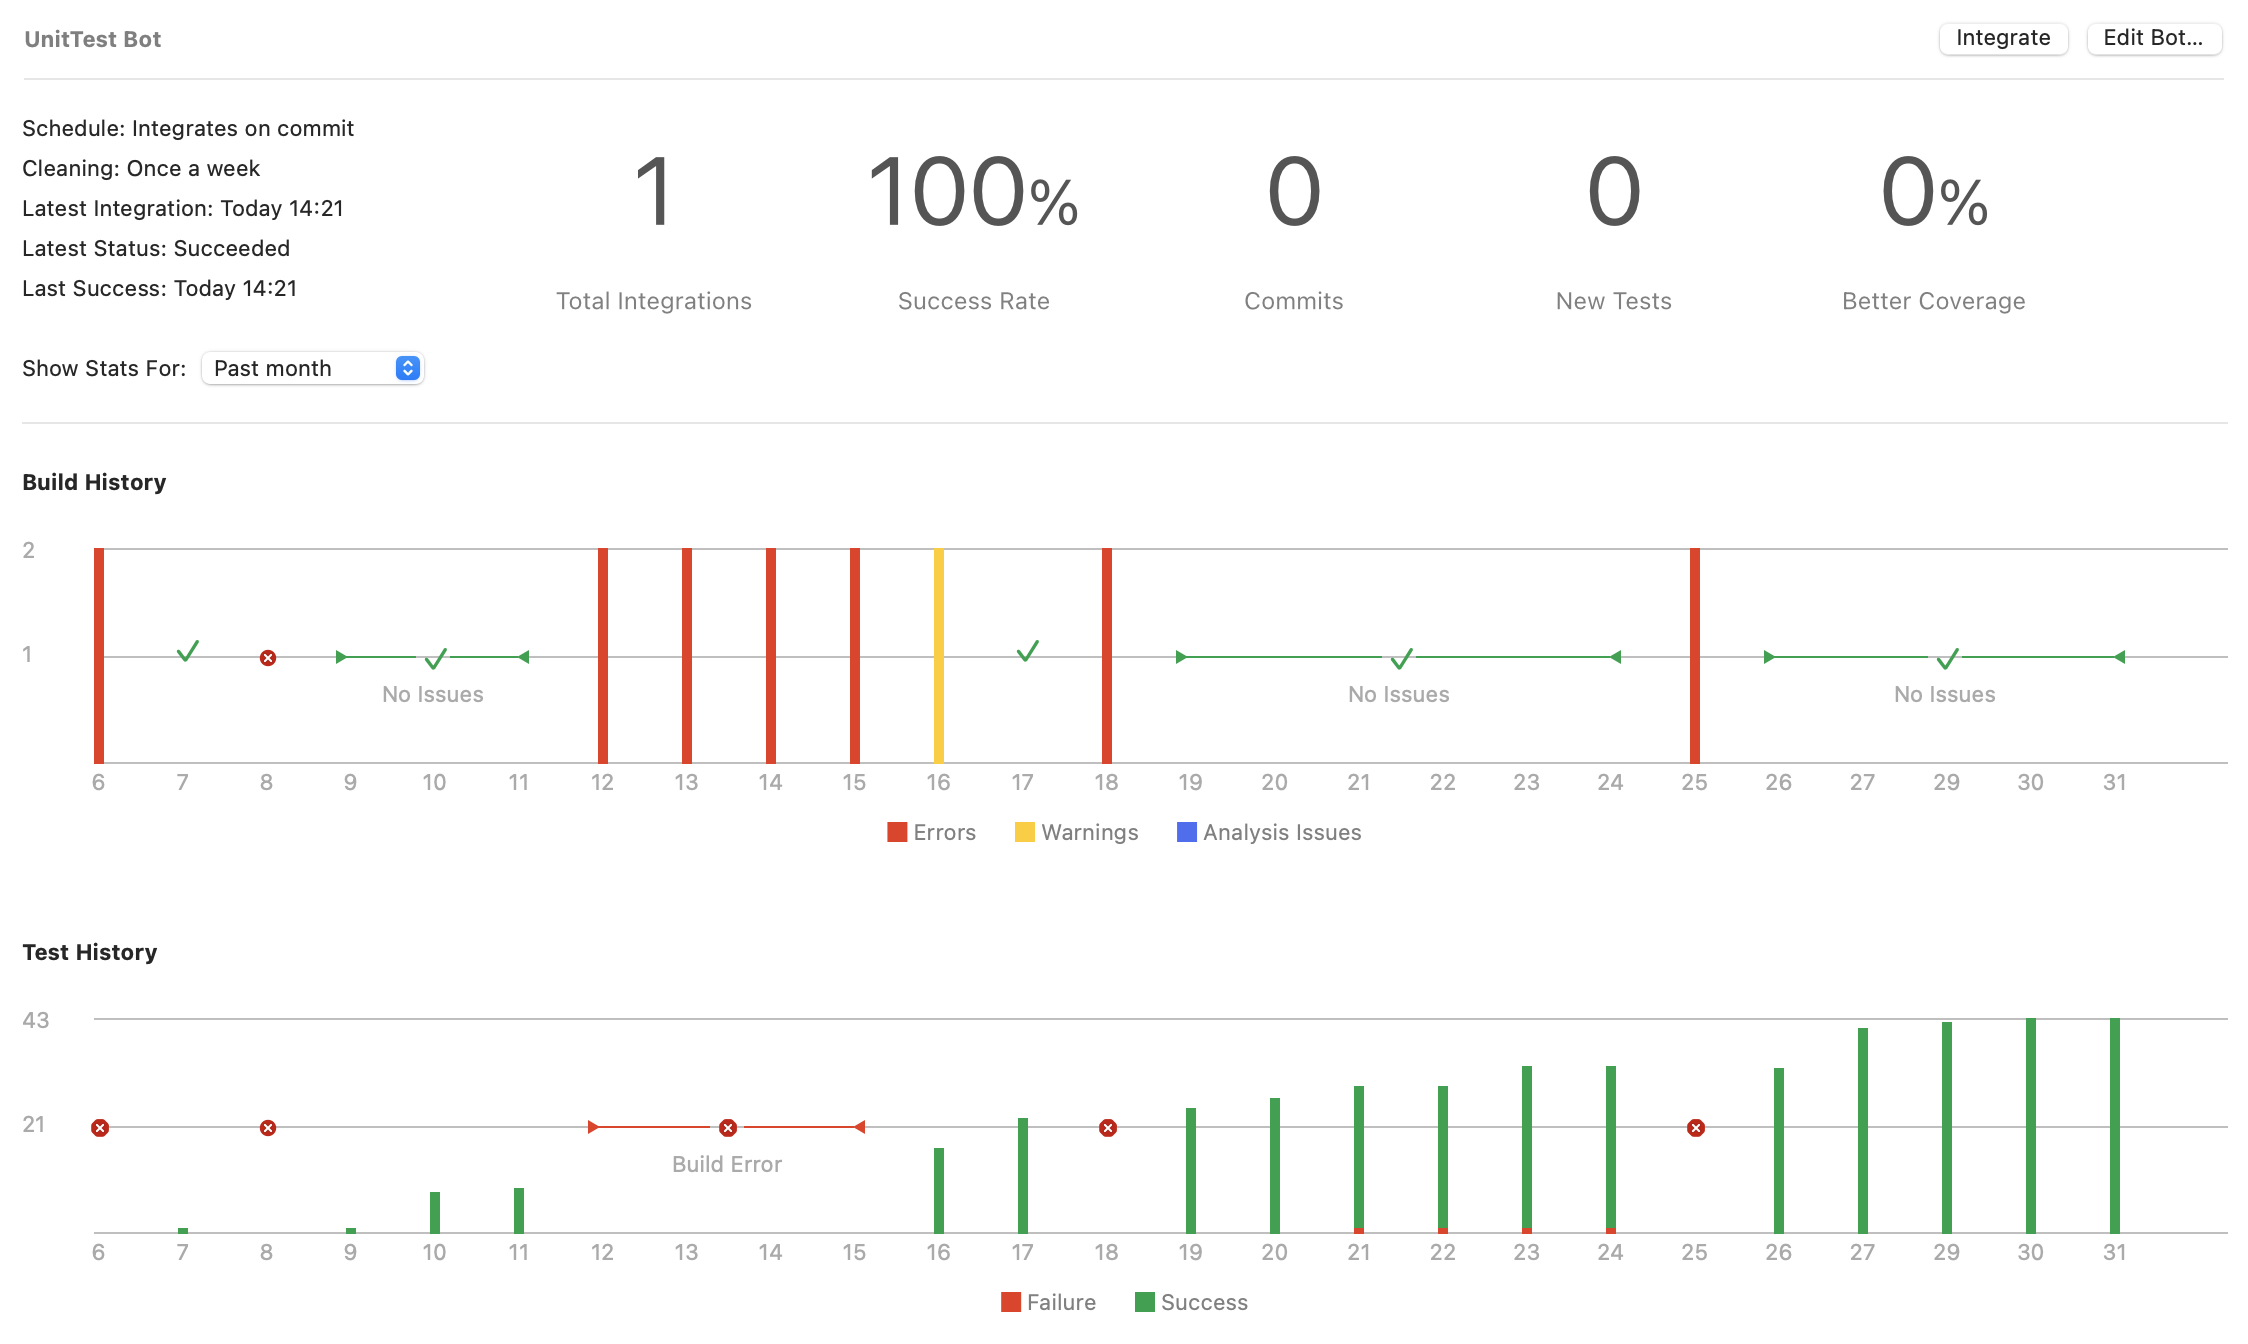
\includegraphics[width=1\textwidth]{img}
  \caption{Painel de integração do \emph{Xcode} \label{fig:int}}
\end{figure}

O \emph{TestBench} e a classe de execução de roteiros foram desenvolvidas com a
interface do \emph{XCTest} em mente e as usam para 
apresentar mensagens de falha quando uma
verificação falha. A Figura~\ref{fig:errmsg} apresenta um exemplo de mensagens de falha
durante a execução de um teste. Na imagem, é possível observar
que, após a subida do \emph{clock} no ciclo oito, o sinal referente ao registrador
$x01$ possuía valor 129 ao invés do esperado de 128, e a falha
foi cascateada em outros erros onde o valor esperado era uma unidade
menor que o valor lido.

\begin{figure}
  \centering
  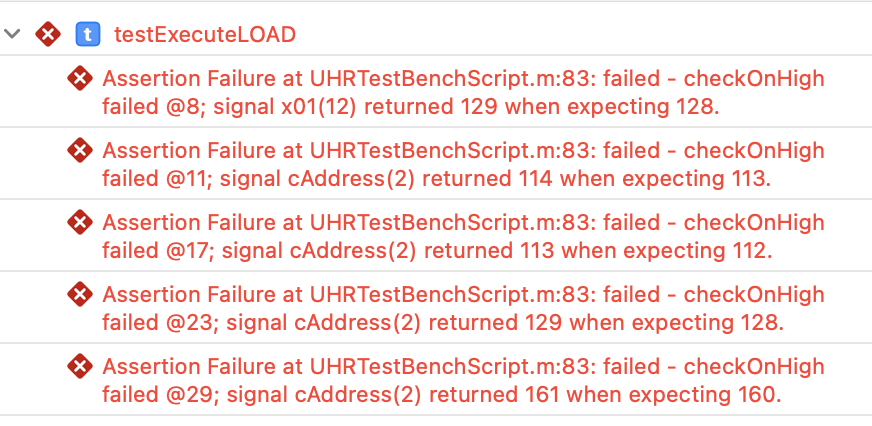
\includegraphics[width=0.5\textwidth]{img2}
  \caption{Exemplo de mensagens de falha de verificação \label{fig:errmsg}}
\end{figure}

\section{Sintetização}
\label{sec:sin}

O processador foi sintetizado para uso em uma placa de desenvolvimento que
utiliza a FPGA \emph{XC7A100T-FGG676ABX1901} da \emph{Xilinx}
e possui o módulo
\emph{CP2102N} da \emph{Silicon Labs} para passar a comunicação UART
através de um cabo USB. A placa também provê um oscilador de cristal
que gera um sinal de \emph{clock} na frequência de 50 \emph{Mhz}, dois botões
e dois diodos emissores de luz.

Para programar a FPGA foi utilizado o \emph{Vivado 2018}, uma suíte
de design da \emph{Xilinx} que possui os programas necessários para
sintetizar a configuração a partir dos módulos e programar o dispositivo.
Além do código em \emph{Verilog}, foi necessário escrever um arquivo
\emph{Xilinx Design Constrain} (XDC) \citep{XDC} que relaciona a entradas e
saídas do módulo de nível mais alto com pinos da FPGA. Com base na folha 
de especificação da placa de desenvolvimento, foi relacionado
quais pinos da \emph{FPGA} representam os dois fios necessários para utilizar o módulo
UART, o gerador de \emph{clock}, os diodos emissores de luz e os botões.
Com base na descrição dos módulos e o arquivo XDC, o \emph{Vivado} gera um arquivo
de configuração. Ao configurar a FPGA com esse arquivo através de uma interface
JTAG, ela passa a funcionar como o processador descrito.


Em relação aos pinos de entrada e saída, o primeiro botão foi mapeado no \emph{bit} 
sB[15][0] e os diodos foram mapeados nos \emph{bits} sB[15][5] e sB[15][4]. Os outros
pinos não foram mapeados em nenhum elemento da placa, e o segundo botão foi mapeado no sinal
de \emph{reset} para inicializar o processador.
Devido a limitação de memória interna da FPGA, foram disponibilizado 
apenas dois bancos de memória para uso na região sD.